\documentclass[unicode,aspectratio=169,11pt]{beamer}
\usepackage{amsmath, amssymb, amsthm, color, latexsym, mathrsfs, bm}
\usefonttheme{professionalfonts}
\usepackage{luatexja}
\usepackage[ipaex]{luatexja-preset}
\renewcommand{\kanjifamilydefault}{\gtdefault}

\usetheme[
  sectionpage=none,
  numbering=fraction,
  block=fill
  ]{metropolis}

\def\qed{\hfill $\Box$}
\def\endexample{\hfill $\clubsuit$}
\newcommand{\ex}{\mathbb{E}}
\newcommand{\var}{\mathrm{var}}
\newcommand{\cov}{\mathrm{cov}}
\newcommand{\bb}{\mathbb}
\newcommand{\cc}{\mathcal}
\newcommand{\tr}{\mathrm{T}}
\newcommand{\trace}{\mathrm{tr}}


\title{6. Random matrices and covariance estimation}
\author{担当:みーとみ}
\date{2021年7月1日, 7月7日}


\begin{document}

\maketitle

\begin{frame}{Table of Contents}{}
    \setcounter{tocdepth}{1}
    \tableofcontents
\end{frame}

\section{6.1 Some preliminaries}
\begin{frame}{6.1 Some preliminaries}
  \begin{itemize}
    \item Notationとこの章で使うpreliminary resultsの説明から.
  \end{itemize}
\end{frame}

\subsection{6.1.1 Notation and basic facts}
\begin{frame}{6.1.1 Notation and basic facts}{}
  \begin{itemize}
    \item 行列 $A \in \bb{R}^{n \times m}$ with $n \ge m$ に対し, (順序付き)特異値を
    \[ \sigma_{\max}(A) = \sigma_1(A) \ge \sigma_2(A) \ge \dots \ge \sigma_m(A) = \sigma_{\min}(A) \ge 0 \]
    と書く.
    \item 最小・最大特異値は次のようにcharacterizeされる:
    \[ \sigma_{\max}(A) = \max_{v \in \bb{S}^{m-1}}\| Av \|_2 \quad \mathrm{and} \quad \sigma_{\min}(A) = \min_{v \in \bb{S}^{m-1}}\|Av\|_2, \tag{6.1} \]
    ただし $\bb{S}^{d-1} := \left\{ v \in \bb{R}^d \mid \|v\|_2 = 1 \right\}$ は $\bb{R}^d$ 上のEuclidean unit sphere.
    \item また次の同値性が成り立つ: $||| A |||_2 = \sigma_{\max}(A)$.
  \end{itemize}
\end{frame}

\begin{frame}
  \begin{itemize}
    \item 対称行列の集合を ${\cc{S}}^{d\times d} := \left\{Q\in\bb{R}^{d\times d} \mid Q = Q^\tr\right\}$ とし, その半正定値行列からなる部分集合を
    \[ \cc{S}_+^{d \times d} := \left\{Q \in \cc{S}^{d \times d} \mid Q \succeq 0\right\} \tag{6.2} \]
    と書く.
    \item 任意の対称行列 $Q \in \cc{S}^{d\times d}$ は対角化可能であり, その固有値を
    \[ \gamma_{\max}(Q) = \gamma_1(Q) \ge \gamma_2 \ge \dots \ge \gamma_d(Q) = \gamma_{\min}(Q) \]
    とする.
    \item このとき, $Q \succeq 0 \ \Leftrightarrow \ \gamma_{\min}(Q) \ge 0$.
  \end{itemize}
\end{frame}

\begin{frame}{}{}
  \begin{itemize}
    \item 最小・最大固有値の ``Rayleigh–Ritz variational characterization'':
    \[
        \gamma_{\max}(Q) = \max_{v \in \bb{S}^{d-1}} v^\tr Q v
        \quad \mathrm{and} \quad
        \gamma_{\min}(Q) = \min_{v \in \bb{S}^{d-1}} v^\tr Q v. \tag{6.3}
    \]
    \item 任意の対称行列 $Q$ に対し, その$\ell_2$-operator normは, 
    \[ |||Q|||_2 = \max \left\{ \gamma_{\max}(Q), |\gamma_{\min}(Q)| \right\} = \max_{v \in \bb{S}^{d-1}}\left|v^\tr Qv\right|.\tag{6.4} \]
    \item 最後に, 行列 $A \in \bb{R}^{n\times m}$ with $n \ge m$ に対し, $m$-次元対称行列 $R := A^\tr A$ を考えると, 
    \[ \gamma_j(R) = \left(\sigma_j(A)\right)^2 \quad \mathrm{for}\ j = 1, \dots, m. \]
  \end{itemize}
\end{frame}

\subsection{6.1.2 Set-up of covariance estimation}
\begin{frame}{6.1.2 Set-up of covariance estimation}{}
  \begin{itemize}
    \item $\{x_1,\dots,x_m\}$ は, $\bb{R}^d$上のzero-mean・covariance $\Sigma = \cov(x_1) \in \bb{S}_+^{d\times d}$なる分布からの $n$ 個のi.i.d.サンプルとする.
    \item $\Sigma$ のstandard estimatorは, 次の {\it sample covariance matrix} である:
    \[ \widehat{\Sigma} := \frac{1}{n}\sum_{i=1}^n x_i x_i^\tr.  \tag{6.5} \]
    \item 各 $x_i$ はzero-meanなので $\ex[x_i x_i^\tr] = \Sigma$ であり, $\widehat{\Sigma}$ は $\Sigma$ のunbiased estimator.
    \item したがって $\widehat{\Sigma}-\Sigma$ は期待値ゼロとなり, その$\ell_2$-operator normによって測ったerrorのboundを求めることがこの章のgoalとなる.
  \end{itemize}
\end{frame}

\begin{frame}
  \begin{itemize}
    \item (6.4) の$\ell_2$-operator normの表現より, $|||\widehat{\Sigma}-\Sigma|||_2 \le \epsilon$ は以下と同値:
    \[ \max_{v \in \bb{S}^{d-1}} \left|\frac{1}{n}\sum_{i=1}^n \langle x_i,v_i \rangle^2 - v^\tr \Sigma v\right| \le \epsilon. \tag{6.6}\]
    \item つまり, $|||\widehat{\Sigma} - \Sigma|||_2$ をコントロールすることは, $v$ でindexedされた関数クラス $x \mapsto \langle x, v\rangle^2$ のuniform law of large numbersを示すことと同値になる.
  \end{itemize}
\end{frame}

\begin{frame}{}{}
 \\
  \begin{itemize}
    \item その$\ell_2$-operator normをコントロールすることは, $\widehat{\Sigma}$ の固有値の一様収束も意味する: Weyl's theorem の corollaryより,
    \[ \max_{j = 1, \dots, d} \left|\gamma_j(\widehat{\Sigma}) - \gamma_j\left(\Sigma\right)\right| \le |||\widehat{\Sigma} - \Sigma|||_2. \tag{6.7} \]
     \\
    \item また最後に, ランダム行列 $X \in \bb{R}^{n \times d}$ が, 第$i$行に $x_i^\tr$ を持つものとする
    \[
      X =
      \begin{pmatrix}
        x_1^\tr\\
        \vdots\\
        x_n^\tr
      \end{pmatrix} \in \bb{R}^{n \times d}
    \]
    と,
    \[ \widehat{\Sigma} = \frac{1}{n}\sum_{i=1}^n x_i x_i^\tr = \frac{1}{n}X^\tr X \]
    なので, $\widehat{\Sigma}$ の固有値は $X / \sqrt{n}$ の特異値の2乗となる.
  \end{itemize}
\end{frame}

\section{6.2 Wishart matrices and their behavior}
\begin{frame}{6.2 Wishart matrices and their behavior}
  \begin{itemize}
    \item サンプル $x_i$ は, $d$-次元正規分布 $\mathcal{N}(0, \Sigma)$ から i.i.d. で引かれるとする.
    \item このとき,
    \[
      X =
      \begin{pmatrix}
        x_1^\tr\\
        \vdots\\
        x_n^\tr
      \end{pmatrix} \in \bb{R}^{n \times d}
    \]
    は, {\it $\Sigma$-Gaussian ensemble} から引かれると言う.
    \item Sample covariance $\widehat{\Sigma} = \frac{1}{n}X^\tr X$ は, {a multivariate Wishart distribution} に従う.
  \end{itemize}
\end{frame}

\begin{frame}{}{}
  \begin{block}{Theorem 6.1}
    $X \in \mathbb{R}^{n \times d}$ は $\Sigma$-Gaussian ensembleから引かれるとする.
    このとき, 任意の $\delta > 0$ に対し, 最大特異値 $\sigma_{\max}(X)$ は以下のupper deviation inequalityを満たす:
    \[
      \bb{P} \left[
        \frac{\sigma_{\max}(X)}{\sqrt{n}}
        \ge \gamma_{\max}\left(\sqrt{\Sigma}\right) (1+\delta) + \sqrt{\frac{\trace(\Sigma)}{n}}
      \right]
      \le \exp\left(-\frac{n\delta^2}{2}\right).
      \tag{6.8}
    \]
    さらに$n \ge d$なら, 最小特異値 $\sigma_{\min}(X)$ は以下のlower deviation inequalityを満たす:
    \[
        \bb{P} \left[
        \frac{\sigma_{\min}(X)}{\sqrt{n}}
        \le \gamma_{\min}\left(\sqrt{\Sigma}\right) (1-\delta) - \sqrt{\frac{\trace(\Sigma)}{n}}
      \right]
      \le \exp\left(-\frac{n\delta^2}{2}\right).
      \tag{6.9}
    \]
  \end{block}
\end{frame}

\begin{frame}{}{}
 \\
{\bf Example 6.2} (Operator norm bounds for the standard Gaussian ensemble)
\begin{itemize}
  \item $W \in \bb{R}^{n \times d}$ は各成分が$\cc{N} (0,1)$ i.i.d.で引かれるrandom matrixとする($\Sigma = I_d$).
  \item Thm 6.1より, $n \ge d$ なら, 確率 $1 - 2 \exp\left(-\frac{n\delta^2}{2}\right)$ 以上で
  \[\frac{\sigma_{\max}(W)}{\sqrt{n}} \le 1 + \delta + \sqrt{\frac{d}{n}}
  \quad \mathrm{and} \quad
  \frac{\sigma_{\min}(W)}{\sqrt{n}} \ge 1 - \delta - \sqrt{\frac{d}{n}}
  \tag{6.10}
  \]
  となる.
  \item よって, 同じ確率で
  \[ \Bigg|\Bigg|\Bigg| \frac{1}{n}W^\tr W - I_d \Bigg|\Bigg|\Bigg|_2 \le 2\epsilon + \epsilon^2,
  \quad \mathrm{where} \epsilon = \sqrt{\frac{d}{n}} + \delta.
  \tag{6.11} \]
  \item したがって, $d/n \to 0$ なら, sample covariance $\widehat{\Sigma} = \frac{1}{n}W^\tr W$ はidentiry matrix $I_d$ の一致推定量となる.\endexample
\end{itemize}
\end{frame}

\begin{frame}{}{}
 \\
{\bf Example 6.3} (Gaussian covariance estimation)
\begin{itemize}
  \item $X \in \bb{R}^{n \times d}$ は$\Sigma$-Gaussian ensembleからのrandom matrixとする.
  \item このとき $X = W \sqrt{\Sigma}$ と書ける($W \in \bb{R}^{n\times d}$はstandard Gaussian random matrix)ので,
          \[
              \Bigg|\Bigg|\Bigg| \frac{1}{n} X^\tr X - \Sigma \Bigg|\Bigg|\Bigg|_2
              = \Bigg|\Bigg|\Bigg|\sqrt{\Sigma}\left(\frac{1}{n}W^\tr W - I_d\right) \Bigg|\Bigg|\Bigg|_2
              \le |||\Sigma|||_2 \Bigg|\Bigg|\Bigg| \frac{1}{n} W^\tr W - I_d \Bigg|\Bigg|\Bigg|_2.
          \]
  \item したがって (6.11) より, 任意の $\delta > 0$ に対して確率 $1 - 2\exp\left(-\frac{n \delta^2}{2}\right)$ で
          \[
            \frac{||| \widehat{\Sigma} - \Sigma |||_2}{|||\Sigma|||_2}
            \le 2 \sqrt{\frac{d}{n}} + 2\delta + \left(\sqrt{\frac{d}{n}} + \delta\right)^2.
            \tag{6.12} 
          \]
  \item よって, $||| \widehat{\Sigma} - \Sigma |||_2 / |||\Sigma|||_2$ は $d/n \to 0$ である限り $0$ に収束する.\endexample
\end{itemize}
\end{frame}

\begin{frame}{}{}
 \\
{\bf Example 6.4} (Faster rates under trace constraints)
\begin{itemize}
  \item $\{ \gamma_j(\Sigma)\}_{j = 1}^d$ は$\Sigma$の固有値列で, $\gamma_1(\Sigma)$ がそのうち最大のもの.
  \item $\Sigma$は, 次元に対して独立な定数 $C$ に対し, 次の ``trace constraint'' を満たすとする:
        \[
            \frac{\trace(\Sigma)}{|||\Sigma|||_2}
            = \frac{\sum_{j=1}^d \gamma_j(\Sigma)}{\gamma_1(\Sigma)}
            \le C.
            \tag{6.13}
        \]
  \item $C$は$\Sigma$の(実質的な)rankと見なせる($\because$ (6.13) は$C = \mathrm{rank}(\Sigma)$では常に成立. )
  \item パラメータ $q \in [0,1]$と半径 $R_q >0$ のthe Schatten $q$-``balls''を, 以下で定義する:
        \[
          \bb{B}_q(R_q)
          := \left\{ \Sigma\in S^{d \times d} \Bigg| \sum_{j=1}^d|\gamma_j(\Sigma)|^q \le R_q \right\}.
          \tag{6.14}
        \]
        \begin{itemize}
          \item $q = 0$なら, rank $R_q$ 以下の対称行列の集合.
          \item $q = 1$なら, trace constraintになる.
        \end{itemize}
  \item 任意の非零行列 $\Sigma \in \bb{B}_q(R_q)$ は, (6.13) を $C = R_q / (\gamma_1(\Sigma))^q$ で満たす.
\end{itemize}
\end{frame}

\begin{frame}{}
\begin{itemize}
  \item (6.13) を満たす任意の$\Sigma$に対し, Thm 6.1は高確率で$X$の最大特異値が次のように抑えられることを保証する:
  \[
      \frac{\sigma_{\max}(X)}{\sqrt{n}} \le \gamma_{\max}(\sqrt{\Sigma}) \left(1 + \delta + \sqrt{\frac{C}{n}}\right).
      \tag{6.15}
  \]
  \item $\Sigma = I_d$のときのbound (6.10) と比べると, $C$ が $d$ に置き換わって``実行的なrank''となっている.\endexample
\end{itemize}
\end{frame}

\begin{frame}{}{}
{\bf Proof of Theorem 6.1.}
\begin{itemize}
  \item Notation: $\overline{\sigma}_{\max} = \gamma_{\max}(\sqrt{\Sigma}),\ \overline{\sigma}_{\min} = \gamma_{\min}(\sqrt{\Sigma})$.
  \item 最大/最小特異値のupper/lower boundともに以下の2段階で示す:
  \begin{enumerate}
    \item 高確率で特異値が期待値に近いことをconcentration inequalityから示す(Ch.2)
    \item その期待値のboundの導出にGaussian comparison inequalityを用いる(Ch.5)
  \end{enumerate}
   \\
  \item ここでは最大特異値のupper boundのみを示す.
        (最小特異値のlower boundは大体似た方針で示せるがよりテクニカルなのでAppendix (Section 6.6)にまわす.)
\end{itemize}
\end{frame}

\begin{frame}
  \begin{itemize}
    \item $X = W \sqrt{\Sigma}$ と書ける, ただし $W \in \bb{R}^{n\times d}$ はi.i.d. $\cc{N}(0,1)$ entriesをもつ.
    \item $W \mapsto \frac{\sigma_{\max}(W\sqrt{\Sigma})}{\sqrt{n}}$ を$\bb{R}^{nd}$上の実数値写像とみると, これは $L = \overline{\sigma}_{\max}/\sqrt{n}$でLipschitz w.r.t. Euclidean norm.(cf. Example 2.32)
    \item Gaussian r.v. に対するLipschitz関数のconcentration inequality(Thm 2.26)より,
          \[
            \bb{P}\left[\sigma_{\max}(X) \ge \ex[\sigma_{\max}(X)] + \sqrt{n} \overline{\sigma}_{\max} \delta\right]
            \le \exp\left(-\frac{n \delta^2}{2}\right).
          \]
    \item したがって, あとは以下を示せれば良い:
          \[
            \ex[\sigma_{\max}(X)] \le \sqrt{n} \overline{\sigma}_{\max} + \sqrt{\trace(\Sigma)}. \tag{6.16}
          \]
  \end{itemize}
\end{frame}

\begin{frame}
  \begin{itemize}
    \item $\sigma_{\max}(X) = \max_{v' \in \bb{S}^{d-1}}\|Xv'\|_2$ で, $X = W\sqrt{\Sigma},\ v = \sqrt{\Sigma}v'$とすると次のように書ける:
          \[
            \sigma_{\max}(X) = \max_{v \in \bb{S}^{d-1}(\Sigma^{-1})} \|W v\|_2
            = \max_{u \in \bb{S}^{d-1}} \max_{v \in \bb{S}^{d-1}(\Sigma^{-1})} \underbrace{u^\tr W v}_{Z_{u,v}},
          \]
          ただし $\bb{S}^{d-1}(\Sigma^{-1}) := \{v \in \bb{R}^d \mid \|\Sigma^{-\frac{1}{2}}v\|_2 = 1\}$.
    \item $\{ Z_{u, v} ,\ (u, v) \in \bb{T}\}$ where $\bb{T} := \bb{S}^{d-1}\times \bb{S}^{d-1}(\Sigma^{-1})$はzero-mean Gaussian processとみなせる.\\
     \\
    \item 別のGaussian process $\{Y_{u,v},\ (u,v)\in \bb{T}\}$ で $\ex[(Z_{u,v}-Z_{\tilde{u}\tilde{v}})^2] \le \ex[(Y_{u,v}-Y_{\tilde{u}\tilde{v}})^2]$
          for all $(u,v), (u',v') \in \bb{T}$ となるようなものをconstructすることを考える.
    \item すると Sudakov-Fernique comparison(Thm. 5.27)から以下が言える:
          \[ \ex[\sigma_{\max}(X)] = \ex\left[\max_{(u,v)\in \bb{T}} Z_{u,v}\right] \le \ex\left[\max_{(u,v)\in \bb{T}} Y_{u,v}\right]. \tag{6.17}\]
  \end{itemize}
\end{frame}

\begin{frame}
  \begin{itemize}
    \item $(u, v), (\tilde{u}, \tilde{v}) \in \bb{T}$ をgivenとし, $\|v\|_2 \le \|\tilde{v}\|_2$とする.
    \item まず$Z_{u,v} =u^\tr W v= \langle\langle W, uv^\tr \rangle\rangle$となる, where $\langle\langle A,B\rangle\rangle := \sum_{j=1}^n\sum_{k=1}^dA_{jk}B_{jk}$.
    \item $W$ はi.i.d.$\cc{N}(0,1)$ entriesをもつので,
          \[
            \ex\left[(Z_{u,v} - Z_{\tilde{u}\tilde{v}})^2\right]
            = \ex \left[\langle\langle W, uv^\tr-\tilde{u}\tilde{v}^\tr\rangle\rangle^2\right]
            = |||uv^\tr - \tilde{u}\tilde{v}^\tr |||^2_F.
          \]
    \item Frobenius normを変形すると,
          \begin{align*}
             &|||uv^\tr - \tilde{u}\tilde{v}^\tr |||^2_F\\
            =&|||u(v - \tilde{v})^\tr - (u-\tilde{u})\tilde{v}^\tr |||^2_F \\
            =&|||(u-\tilde{u})\tilde{v}^\tr|||^2_F + |||u(v-\tilde{v})-\tr|||^2_F + 2\langle\langle u(v-\tilde{v})^\tr, (u-\tilde{u})\tilde{v}^\tr\rangle\rangle\\
            \le& \|\tilde{v}\|_2^2\|u-\tilde{u}\|_2^2 + \|u\|_2^2\|v-\tilde{v}\|_2^2 + 2(\|u\|_2^2-\langle u,\tilde{u}\rangle)(\langle v,\tilde{v}\rangle-\|\tilde{v}\|_2^2).
          \end{align*}
    \item ここで, $\|u\|_2 = \|\tilde{u}\|_2 = 1$ より $\|u\|_2^2 - \langle u, \tilde{u}\rangle \ge 0$.
    \item 一方, Cauchy-Schwarzと仮定$\|v\|_2 \le \|\tilde{v}\|_2$より, $|\langle v, \tilde{v}\rangle| \le \|v\|_2 \|\tilde{v}\|_2 \le \|\tilde{v}\|_2^2$.
    \item したがって, 
          \[|||uv^\tr - \tilde{u}\tilde{v}^\tr |||^2_F \le  \|\tilde{v}\|_2^2\|u-\tilde{u}\|_2^2 + \|v-\tilde{v}\|_2^2.\]
  \end{itemize}
\end{frame}

\begin{frame}
  \begin{itemize}
    \item $\bb{S}^{d-1}(\Sigma^{-1})$の定義より, $\|\tilde{v}\|_2 \le \overline{\sigma} = \gamma_{\max}(\sqrt{\Sigma})$ なので,
            \[ \ex[(Z_{u,v} - Z_{\tilde{u}, \tilde{v}})^2] \le \overline{\sigma}^2_{\max} \|u-\tilde{u}\|_2^2 + \|v-\tilde{v}\|_2^2.\]
    \item Gaussian process $Y_{u,v} := \overline{\sigma}_{\max}\langle g, u\rangle + \langle h, v\rangle$ を定義する(ただし $g\in\bb{R}^n, h \in \bb{R}^d$ はstandard Gaussian rv's)と,
            \[ E[(Y_{u,v} - Y_{\tilde{u},\tilde{v}})^2] = \overline{\sigma}^2_{\max}\|u-\tilde{u}\|_2^2 + \|v - \tilde{v}\|_2^2. \]
    \item よって Sudakov-Fernique bound (6.17) より,
    \begin{align*}
      \ex[\sigma_{\max}(X)] \le \ex\left[ \sup_{(u,v) \in \bb{T}} Y_{u,v}\right]
      &= \overline{\sigma}_{\max}\ex\left[\sup_{u \in\bb{S}^{d-1}}\langle g, u \rangle\right] + \ex\left[ \sup_{v \in \bb{S}^{d-1}(\Sigma^{-1})}\langle h, v\rangle \right]\\
      &= \overline{\sigma}_{\max}\ex[\|g\|_2] + \ex[\|\sqrt{\Sigma}h\|_2].
    \end{align*}
    \item Jensen's inequalityから, $\ex[\|g\|_2] \le \sqrt{n}$ ans $\ex[\|\sqrt{\Sigma}h\|_2] \le \sqrt{\ex[h^\tr \Sigma h]} = \sqrt{\trace(\Sigma)}$となり, (6.16)が示された.\qed
  \end{itemize}
\end{frame}

\section{6.3 Covariance matrices from sub-Gaussian ensembles}
\begin{frame}{6.3 Covariance matrices from sub-Gaussian ensembles}{}
  \begin{itemize}
    \item Random vector $x_i \in \bb{R}^d$ はzero-meanで, sub-Gaussian with parameter at most $\sigma$, つまり各 $v \in \bb{S}^{d-1}$ に対し,
          \[
              \ex\left[\exp\left(\lambda \langle v, x_i \rangle\right)\right]
              \le \exp\left(\frac{\lambda^2\sigma^2}{2}\right)
              \quad \mathrm{for\ all}\ \lambda \in \bb{R}
              \tag{6.18}
          \]
          が成り立つとする.
          \begin{itemize}
            \item 例1) $x_{ij} \in \bb{R}$ はzero-mean, sub-Gaussian with $\sigma = 1$\\
                  ($x_{ij} \sim \cc{N}(0,1)$やRademacher variable, サポート$[-1,1]$の分布など)
            \item 例2) $x_i \sim \cc{N}(0, \Sigma)$ とすると,
            任意の $v \in \bb{S}^{d-1}$ に対し $\langle v, x_i \rangle \sim \cc{N}(0, v^\tr \Sigma v)$ で $v^\tr \Sigma v \le |||\Sigma|||_2$ より,
            $x_i$ は sub-Gaussian with parameter at most $\sigma^2 = |||\Sigma|||_2$.
          \end{itemize}
    \item このとき, $X \in \bb{R}^{n \times d}$ は {\it row-wise $\sigma$-sub-Gaussian ensemble} からのサンプルであるという.
  \end{itemize}
\end{frame}

\begin{frame}
  \begin{block}{Theorem 6.5}
    ある定数 $c_0, c_1, c_2 , c_3$ が存在して,
    任意のrow-wise $\sigma$-sub-Gaussianランダム行列 $X \in \bb{R}^{n \times d}$ について,
    標本共分散 $\widehat{\Sigma} = \frac{1}{n}\sum_{i=1}^n x_i x_i^\tr$ は次ののbound
    \[
      \ex\left[ \exp\left( \lambda |||\widehat{\Sigma} - \Sigma|||_2 \right) \right]
      \le \exp\left( c_0\frac{\lambda^2\sigma^2}{n} + 4d \right)
      \quad \mathrm{for\ all}\ |\lambda| < \frac{n}{64e^2\sigma^2}
      \tag{6.19a}
    \]
    を満たし, したがって,
    \[
      \bb{P}\left[ \frac{|||\widehat{\Sigma} - \Sigma|||_2}{\sigma^2} \ge c_1 \left\{ \sqrt{\frac{d}{n}} + \frac{d}{n} \right\} + \delta \right]
      \le c_2 \exp\left(-c_3 n \min\{\delta, \delta^2\}\right)
      \quad \mathrm{for\ all}\ \delta \ge 0.
      \tag{6.19b}
    \]
  \end{block}
\end{frame}

\begin{frame}{}{}
   \\
  {\it Remarks:}
  \begin{itemize}
    \item (6.19a) をgivenとすると, Chernoff technique (Ch.2) からただちに (6.19b) が示される.
    \item $\Sigma = I_d$ で $x_i$ がsub-Gaussian w/ $\sigma = 1$のとき, (6.19b)は高確率で
          \[ |||\widehat{\Sigma} - I_d|||_2 \precsim \sqrt{\frac{d}{n}}+\frac{d}{n}\]
          となることを含意する.
    \item $n \ge d$ のとき, これは定数 $c' > 1$ について
          \[
            1 - c' \sqrt{\frac{d}{n}}
            \le \frac{\sigma_{\min}(X)}{\sqrt{n}}
            \le \frac{\sigma_{\max}(X)}{\sqrt{n}}
            \le 1 + c' \sqrt{\frac{d}{n}}
            \tag{6.20}
          \]
          を意味し, standard Gaussian matrixについてのresult (6.10) の sub-Gaussian versionとみなせる.
  \end{itemize}
\end{frame}

\begin{frame}{}{}
  {\bf Proof}
  \begin{itemize}
    \item $Q := \widehat{\Sigma} - \Sigma$ の $\ell_2$-operator normのmoment母関数のboundを求めたい.
    \item まずSection 6.1より $||| Q |||_2 = \max_{v \in \bb{S}^{d-1}} |\langle v, Qv \rangle|$.
    \item Example 5.8より, $\bb{S}^{d-1}$ には$N (\le 17^d)$個のベクトルからなる $\frac{1}{8}$-covering が存在し, これを $\{v^1 ,\dots, v^N\}$ とかく.
    \item 任意の $v \in \bb{S}^{d-1}$ は $v = v^j + \Delta$ where $\|\Delta\|_2 \le \frac{1}{8}$ とかけ, よって
            \[
              \langle v, Qv \rangle
              = \langle v^j, Qv^j \rangle + 2\langle \Delta, Qv^j \rangle + \langle \Delta, Q\Delta \rangle.
            \]
    \item 三角不等式とoperator normの定義から
            \begin{align*}
              |\langle v, Qv \rangle|
              &\le |\langle v^j, Qv^j \rangle| + 2\|\Delta\|_2 |||Q|||_2 \|v^j\|_2 + |||Q|||_2\|\Delta\|_2^2\\
              &\le |\langle v^j, Qv^j \rangle| + \frac{1}{4} |||Q|||_2 + \frac{1}{64} |||Q|||_2\\
              &\le |\langle v^j, Qv^j \rangle| + \frac{1}{2}|||Q|||_2.
            \end{align*}
  \end{itemize}
\end{frame}

\begin{frame}
  \begin{itemize}
    \item $v \in \bb{S}$ について$\sup$をとると,
            \[ |||Q|||_2 = \max_{v \in \bb{S}^{d-1}} |\langle v, Qv\rangle| \le 2 \max_{j = 1,\dots,N} |\langle v^j, Qv^j\rangle|. \]
    \item よって,
            {\small
            \[
                \ex\left[e^{\lambda|||Q|||_2}\right]
                \le \ex\left[\exp\left( 2\lambda\max_{j=1,\dots,N}|\langle v^j, Qv^j \rangle| \right)\right]
                \le \sum_{j=1}^N\left\{ \ex\left[e^{2\lambda\langle v^j, Qv^j\rangle}\right] + \ex\left[e^{-2\lambda\langle v^j, Qv^j\rangle}\right] \right\}.
                \tag{6.21}
            \]}
    \item ここで, 任意の $u \in \bb{S}^{d-1}$ に対して以下が成り立つ(証明は後で):
            \[
              \ex\left[ e^{t \langle u, Qu \rangle} \right] \le e^{512 \frac{t^2}{n} e^4 \sigma^4} 
              \quad \mathrm{for\ all}\ |t| \le \frac{n}{32 e^2 \sigma^2}.
              \tag{6.22}
            \]
    \item (6.21) (6.22) より,
            \[
                \ex\left[e^{\lambda |||Q|||_2}\right] \le 2Ne^{2048 \frac{\lambda^2}{n}e^4 \sigma^4} \le \exp\left(c_0 \frac{\lambda^2\sigma^4}{n}+4d\right)
                \quad \mathrm{for\ all}\ |\lambda| < \frac{n}{64 e^2 \sigma^2}
            \]
            となり(2つ目の不等号は$2\cdot 17^d \le e^{4d}$より) , (6.19a) が示された.
  \end{itemize}
\end{frame}

\begin{frame}{}{}
  {\it Proof of the bound (6.22)}
  \begin{itemize}
    \item $Q = \widehat{\Sigma} - \Sigma$ の定義とi.i.d.の仮定より,
          \begin{align*}
            \ex\left[e^{t\langle u, Qu\rangle}\right]
            = \prod_{i=1}^n \ex\left[e^{\frac{t}{n}\left\{\langle x_i, u\rangle^2 - \langle u, \Sigma u\rangle\right\}}\right]
            = \left( \ex\left[e^{\frac{t}{n}\left\{\langle x_1, u\rangle^2 - \langle u, \Sigma u\rangle\right\}}\right] \right)^n.
            \tag{6.23}
          \end{align*}
    \item $\epsilon \in \{-1, 1\}$をRademacher変数とすると, symmetrization argument (Prop.4.11)より
          \begin{align*}
            \mathbb{E}_{x_{1}}\left[e^{\frac{t}{n}\left\{\left\langle x_{1}, u\right\rangle^{2}-\langle u, \Sigma u\rangle\right\}}\right]
            \leq \mathbb{E}_{x_{1}, \varepsilon}\left[e^{\frac{2 t}{n} \varepsilon\left\langle x_{1}, u\right\rangle^{2}}\right]
            & \stackrel{(\mathrm{i})}{=} \sum_{k=0}^{\infty} \frac{1}{k !}\left(\frac{2 t}{n}\right)^{k} \mathbb{E}\left[\varepsilon^{k}\left\langle x_{1}, u\right\rangle^{2 k}\right] \\
            & \stackrel{(\mathrm{ii})}{=} 1+\sum_{\ell=1}^{\infty} \frac{1}{(2 \ell) !}\left(\frac{2 t}{n}\right)^{2 \ell} \mathbb{E}\left[\left\langle x_{1}, u\right\rangle^{4 \ell}\right]
          \end{align*}
          となる, ただし(i)は指数関数の冪乗展開, (ii)は奇数次項はRademacher termが$0$になることより.
  \end{itemize}
\end{frame}

\begin{frame}{}{}
  \begin{itemize}
    \item Thm.2.6のsub-Gaussianの同値条件より,
            \[
              \ex\left[ \langle x_1, u\rangle^{4\ell} \right]
              \le \frac{(4\ell)!}{2^{2\ell}(2\ell)!}(\sqrt{8}e\sigma)^{4\ell}
              \quad \mathrm{for\ all}\ \ell = 1,2,\dots,
            \]
            が成り立つので,
            \begin{align*}
              \mathbb{E}_{x_{1}}\left[e^{\frac{t}{n}\{\left\langle x_{1}, u\right\rangle^{2}-\langle u, \Sigma u\rangle\}}\right] & \leq 1+\sum_{\ell=1}^{\infty} \frac{1}{(2 \ell) !}\left(\frac{2 t}{n}\right)^{2 \ell} \frac{(4 \ell) !}{2^{2 \ell}(2 \ell) !}(\sqrt{8} e \sigma)^{4 \ell} \\
              & \leq 1+\sum_{\ell=1}^{\infty}\Bigg(\underbrace{\frac{16 t}{n} e^{2} \sigma^{2}}_{f(t)}\Bigg)^{2 \ell}
            \end{align*}
            となる, ただし最後の不等号は$(4\ell)! \le 2^{2\ell}[(2\ell)!]^2$より.
  \end{itemize}
\end{frame}

\begin{frame}{}{}
  \begin{itemize}
    \item $f(t) = \frac{16t}{n}e^2 \sigma^2 < \frac{1}{2}$なら
      \[1+\sum_{\ell=1}^{\infty}\left[f^{2}(t)\right]^{\ell} = \frac{1}{1-f^{2}(t)} \stackrel{(\mathrm{i})}{\leq} \exp \left(2 f^{2}(t)\right)\]
      となる((i)は$1/(1-a) \le e^{2a}\mathrm{\ for\ all\ }a \in [0,1/2]$より)ので,
      (6.23)と合わせて $|t| < \frac{n}{32 e^2 \sigma^2}$ に対して $\ex[e^{t \langle u, Qu \rangle}] \le e^{2nf^2(t)}$, つまり(6.22)が示された.\qed
  \end{itemize}
\end{frame}

\begin{frame}{6.4 Bounds for general matrices}{}
  \begin{itemize}
    \item より一般的な条件下でのboundを求める.
    \item そのために covariance matrices だけでなくよりgeneralなrandom matricesを考える.
    \item Main resultのTheorem 6.15と6.17はHoeffding・Bernstein boundsのmatrix-based analogsである.
  \end{itemize}
\end{frame}

\begin{frame}{6.4.1 Background on matrix analysis}{}
   \\
  \begin{itemize}
    \item 対称行列$Q \in \cc{S}^{d\times d}$の対角化$Q = U^\tr \Gamma U$を考える:
    \begin{itemize}
      \item $U \in \bb{R}^{d\times d}$はユニタリ行列 $U^\tr U = I_d$.
      \item $\Gamma := \mathrm{diag}(\gamma(Q))$は固有値 $\gamma(Q) \in \bb{R}^d$からなる対角行列.
    \end{itemize}
     \\
    \item 関数 $f : \bb{R} \to \bb{R}$ を $\cc{S}^{d\times d}$上の関数に以下のように拡張する:
          \[
              Q \mapsto f(Q) := U^\tr \mathrm{diag}(f(\gamma_1(Q)), \dots, f(\gamma_d(Q))) U.
          \]
          \begin{itemize}
            \item このとき, $f$はユニタリ不変, つまり
                  \[ f(V^\tr Q V) = V^\tr f(Q) V \quad \mathrm{for\ all\ unitary\ matrices\ } V \in \bb{R}^{d\times d}. \]
            \item また, 固有値は次のように変換される({\it spectral mapping property}):
                  \[ \gamma(f(Q)) = \{ f(\gamma_j(Q)),\ j=1,\dots,d \}. \]
          \end{itemize}
  \end{itemize}
\end{frame}

\begin{frame}
   \\
  \begin{itemize}
    \item 特に matrix exponential と matrix logarithm の2つの関数がこの章では重要.
    \item Matrix exponential:
    \begin{itemize}
      \item Power-series expansionが成立: $e^Q = \sum_{k = 0}^\infty \frac{Q^k}{k!}$.
      \item Spectral mapping propertyより, $e^Q$ の固有値は常に正, よって $e^Q$は常に正定値.
    \end{itemize}
    \item Matrix logarithmはmatrix exponentialのinverse.\\
     \\
    \item 関数 $f$ が単調であるとは, $Q \preceq R$ ならば $f(Q) \preceq f(R)$ が成り立つことをいう.
    \item Matrix logarithmは単調である(Lowner-Heinz theorem)
    \item Matrix exponentialは単調でない.\\
     \\
    \item $f : \bb{R} \to \bb{R}$が連続かつ非減少なら, 任意の対称行列$Q \preceq R$ に対し,
          \[ \trace(f(Q)) \le \trace(f(R)) \tag{6,25}\]
          が成り立つ({\it trace inequality}).
  \end{itemize}
\end{frame}

\begin{frame}{6.4.2 Tail conditions for matrices}{}
  \begin{itemize}
    \item 対称ランダム行列$Q \in \cc{S}^{d\times d}$に対し, polynomial moment $\ex[Q^j]$ が存在すると仮定する.
    \item $Q$のvarianceは $\var(Q) := \ex[Q^2] - (\ex[Q])^2$で, これは半正定値(Ex.6.6)
    \item $Q$のmoment generating function $\Psi_Q:\bb{R} \to \cc{S}^{d\times d}$は以下で与えられる:
          \[
            \Psi_Q(\lambda) := \ex[e^{\lambda Q}] = \sum_{k=0}^\infty \frac{\lambda^k}{k!} \ex[Q^k].
            \tag{6.26}
          \]
    \item Ch.2の議論と同様に, このmoment generating functionを用いてrandom matrixのsub-Gaussianとsub-exponentialが定義される.
  \end{itemize}
\end{frame}

\begin{frame}{}{}
  \begin{block}{Definition 6.6}
    Zero-mean対称ランダム行列$Q \in \cc{S}^{d\times d}$がsub-Gaussian with matrix parameter $V \in \cc{S}_{+}^{d \times d}$であるとは,
    以下が成り立つことをいう:
    \[
      \Psi_Q(\lambda) \preceq e^{\frac{\lambda^2 V}{2}}
      \quad \mathrm{for\ all}\ \lambda \in \bb{R}.
      \tag{6.27}
    \]
  \end{block}
  {\bf Example 6.7}
  \begin{itemize}
    \item $Q = \epsilon B$で, $\epsilon \in \{-1, 1\}$はRademacher変数, $B \in \cc{S}^{d \times d}$はfixed matrixとする.
    \item このとき, $\ex[Q^{2k+1}] = 0$かつ$\ex[Q^{2k}] = B^{2k}$なので, 
          \[
            \ex[e^{\lambda Q}]
            = \sum_{k=0}^\infty\frac{\lambda^{2k}}{(2k)!}B^{2k}
            \preceq \sum_{k=1}^\infty \frac{1}{k!} \left(\frac{\lambda^2 B^2}{2}\right)^k
            = e^{\frac{\lambda^2 B^2}{2}}
          \]
          となり, $Q$はsub-Gaussian w/ $V = B^2 = \var(Q)$.
    \item より一般に, $Q = gB$で$g \in \bb{R}$がzero-mean $\sigma$-sub-Gaussianなら, $Q$は$V = \sigma^2 B^2$でsub-Gaussianとなる.\endexample
  \end{itemize}
\end{frame}

\begin{frame}{}{}
  {\bf Example 6.8}
  \begin{itemize}
    \item $Q = \epsilon C$で, $\epsilon$はRademacher変数, $C$は$\epsilon$と独立で$|||C|||_2 \le b$なるランダム行列とする.
    \item まず$C$を固定して$\epsilon$について期待値をとると$\ex_\epsilon[e^{\lambda \epsilon C}] \preceq e^{\frac{\lambda^2}{2}C^2}$.
    \item さらに$||| C |||_2 \le b$より $e^{\frac{\lambda^2}{2}C^2} \preceq e^{\frac{\lambda^2}{2}b^2 I_d}$ となり, よって
          \[ \Psi_Q(\lambda) \preceq e^{\frac{\lambda^2}{2}b^2 I_d} \quad \mathrm{for\ all}\ \lambda \in \bb{R}.\]
    \item したがって, $Q$はsub-Gaussian w/ matrix parameter $V = b^2 I_d$.\endexample
  \end{itemize}
\end{frame}

\begin{frame}{}{}
  \begin{block}{Definition 6.9}
    Zero-meanランダム行列$Q$が sub-exponential with parameters $(V, \alpha)$であるとは, 以下が成り立つことをいう:
    \[
        \Psi_Q(\lambda) \preceq e^{\frac{\lambda^2 V}{2}} \quad \mathrm{for\ all}\ |\lambda| < \frac{1}{\alpha}.
        \tag{6.28}
    \]
  \end{block}
  \begin{itemize}
    \item 任意のsub-Gaussian行列はsub-exponential w/ $(V, 0)$.
    \item Sub-exponentialだがsub-Gaussianでないランダム行列はありうる:
    \begin{itemize}
      \item 例)$M = \epsilon g^2 B$ where $\epsilon$はRademacher変数, $g \sim \cc{N}(0, 1)$ でそれぞれ独立.
    \end{itemize}
  \end{itemize}
\end{frame}

\begin{frame}
  \begin{itemize}
    \item Sub-exponentialの1つの判定方法は, 次のBernstein conditionである.
  \end{itemize}
  \begin{block}{Definition 6.10 (Bernstein's condition for matrices)}
    Zero-mean対称ランダム行列$Q$がBernstein condition with parameter $b >0$ を満たすとは, 以下が成り立つことをいう.
    \[
      \ex[Q^j] \preceq \frac{1}{2}j! b^{j-2} \var(Q) \quad \mathrm{for}\ j=3,4,\dots .
      \tag{6.29}
    \]
  \end{block}
  \begin{itemize}
    \item $Q$がbounded operator normを持つ, つまり $|||Q|||_2 \le b$ almost surely の場合, 次が成り立つ.
          \[ \ex[Q^j] \preceq b^{j - 2} \var(Q) \quad \mathrm{for\ all}\ j=3,4,\dots.\tag{6.30} \]
  \end{itemize}
\end{frame}

\begin{frame}{}{}
  \begin{itemize}
    \item 次のLemmaは, Bernstein conditionがsub-exponential conditionを含意することを示す.
  \end{itemize}
  \begin{block}{Lemma 6.11}
    Bernstein conditionを満たす任意のzero-mean対称行列に対し, 以下が成り立つ:
    \[
      \Psi_Q(\lambda) \preceq \exp\left( \frac{\lambda^2 \var(Q)}{2(1 - b |\lambda|)} \right)
      \quad \mathrm{for\ all}\ |\lambda| < \frac{1}{b}.
      \tag{6.31}
    \]
  \end{block}
\end{frame}

\begin{frame}{}{}
   \\
  {\bf Proof}
  \begin{itemize}
    \item $\ex[Q] = 0$なので, matrix exponentialのpower-series expansionより
          \begin{align*}
            \ex[e^{\lambda Q}] 
            &= I_d + \frac{\lambda^2 \var(Q)}{2} + \sum_{j=3}^\infty \frac{\lambda^j \ex[Q^j]}{j!}\\
            &\stackrel{(\mathrm{i})}{\preceq} I_d + \frac{\lambda^2 \var(Q)}{2}\left\{\sum_{j=0}^\infty |\lambda|^jb^j\right\}\\
            &\stackrel{(\mathrm{ii})}{=} I_d + \frac{\lambda^2 \var(Q)}{2(1 - b|\lambda|)} \\
            &\stackrel{(\mathrm{iii})}{\preceq} \exp\left( \frac{\lambda^2 \var(Q)}{2(1 - b|\lambda|)} \right),
          \end{align*}
          ただし(i)はBernstein condition, (ii)は$|\lambda| < 1/b$で成立, (iii)はmatric inequality $I_d + A \preceq e^A$ (for any symmetric matrix $A$)より.
  \end{itemize} 
\end{frame}

\subsection{6.4.3 Matrix Chernoff approach and independent decompositions}

\begin{frame}{6.4.3 Matrix Chernoff approach and independent decompositions}
  \begin{itemize}
    \item まず Chernoff approach の matrix バージョンから.
  \end{itemize}
  \begin{block}{Lemma 6.12 (Matrix Chernoff technique)}
    $Q$ はzero-mean symmetric random matrixで,
    そのmoment generating function $\Psi_Q$ は $\lambda \in (-a, a)$ の範囲で存在するものとする.
    このとき, 任意の$\delta > 0$ に対して以下が成り立つ:
    \[
      \mathbb{P}\left[\gamma_{\max }( {Q}) \geq \delta\right]
      \leq \operatorname{tr}\left(\Psi_{ {Q}}(\lambda)\right) e^{-\lambda \delta} \quad \text { for all } \lambda \in[0, a).
    \tag{6.32}
    \]
    さらに同様に,
    \[
      \mathbb{P}\left[\| {Q}\|_{2} \geq \delta\right]
      \leq 2 \operatorname{tr}\left(\Psi_{ {Q}}(\lambda)\right) e^{-\lambda \delta} \quad \text { for all } \lambda \in[0, a).
      \tag{6.33}
    \]
  \end{block}
\end{frame}

\begin{frame}{}{}
   \\
{\bf Proof}
\begin{itemize}
  \item 各 $\lambda \in [0, a)$ に対し, まず以下が成り立つ.
        \[
          \mathbb{P}\left[\gamma_{\max }( {Q}) \geq \delta\right]
          =\mathbb{P}\left[e^{\gamma_{\max }(\lambda  {Q})} \geq e^{\lambda \delta}\right]
          \stackrel{(\mathrm{i})}{=} \mathbb{P}\left[\gamma_{\max }\left(e^{\lambda  {Q}}\right) \geq e^{\lambda \delta}\right],
          \tag{6.34}
        \]
        ただし(i)は行列関数の固有値の変換(spectral mapping property)から.
  \item Marlkov's inequalityより,
        \[
          \mathbb{P}\left[\gamma_{\max }\left(e^{\lambda  {Q}}\right) \geq e^{\lambda \delta}\right]
          \leq \mathbb{E}\left[\gamma_{\max }\left(e^{\lambda  {Q}}\right)\right] e^{-\lambda \delta}
          \stackrel{\mathrm{(i)}}{\leq} \mathbb{E}\left[\operatorname{tr}\left(e^{\lambda  {Q}}\right)\right] e^{-\lambda \delta}
          \tag{6.35}
        \]
        ただし(i)は$e^{\lambda Q}$がpositive definiteから $\gamma_{\max} (e^{\lambda Q}) \le \trace(e^{\lambda Q})$.
  \item Traceと$\ex$は交換可能なので,
        \[
          \mathbb{E}\left[\operatorname{tr}\left(e^{\lambda  {Q}}\right)\right]
          =\operatorname{tr}\left(\mathbb{E}\left[e^{\lambda  {Q}}\right]\right)
          =\operatorname{tr}\left(\Psi_{ {Q}}(\lambda)\right).
        \]
  \item 同じことが $\gamma(-Q) \ge \delta$, つまり $\gamma_{\min}(Q) \le -\delta$ にも成り立ち,
        $|||Q|||_2 = \max\{\gamma_{\max}(Q) |\gamma_{\min}(Q)|\}$なので, (6.33)も成り立つ.\qed
\end{itemize}
\end{frame}

\begin{frame}{}{}
  \begin{block}{Lemma 6.13}
    $Q_1,\dots,Q_n$は独立な対称ランダム行列で, moment generating functionは$\lambda \in I$に対し存在するものとし,
    $S_n := \sum_{i=1}^n Q_i$とする.
    このとき以下が成り立つ.
    \[
      \operatorname{tr}\left(\Psi_{\mathrm{S}_{n}}(\lambda)\right)
      \leq \operatorname{tr}\left(e^{\sum_{i=1}^{n} \log \Psi_{Q_i}(\lambda)}\right) \quad \text { for all } \lambda \in I.
      \tag{6.36}
    \]
  \end{block}
  {Remark:}
  \begin{itemize}
    \item Lemma 6.12とあわせると, 独立なランダム行列の和のoperator normのtail boundが得られる, つまり, 
          \[
            \mathbb{P}\left[\left|\left|\left|\frac{1}{n} \sum_{i=1}^{n} \mathbf{Q}_{i}\right|\right|\right|_{2} \geq \delta\right]
            \leq 2 \operatorname{tr}\left(e^{\sum_{i=1}^{n} \log \Psi_{Q_i}(\lambda)}\right) e^{-\lambda n \delta}
            \quad \text { for all } \lambda \in[0, a).
          \]
  \end{itemize}
\end{frame}

\begin{frame}{}{}
   \\
{\bf Proof.}
\begin{itemize}
  \item Lieb(1973) より次のresultを用いる: 任意のfixed matrix $H \in S^{d\times d}$に対し, 次の関数 $f : S^{d\times d}_+ \to \bb{R}$
        \[ f(A) := \trace(e^{H + \log(A)}) \]
        はconcaveである.
  \item $G(\lambda) := \trace(\Psi_{S_n}(\lambda))$とかくと, traceと期待値の線形性から
        \[
          G(\lambda)
          =\operatorname{tr}\left(\mathbb{E}\left[e^{\lambda \mathbf{S}_{n-1}+\log \exp \left(\lambda \mathbf{Q}_{n}\right)}\right]\right)
          =\mathbb{E}_{\mathbf{S}_{n-1}} \mathbb{E}_{\mathbf{Q}_{n}}\left[\operatorname{tr}\left(e^{\lambda \mathbf{S}_{n-1}+\log \exp \left(\lambda \mathbf{Q}_{n}\right)}\right)
          \right].
        \]
  \item $H = \lambda S_{n-1},\ A = e^{\lambda Q_n}$としたときの$f$のconcavityとJensen's inequalityより,
        \[
          \mathbb{E}_{\mathbf{Q}_{n}}\left[\operatorname{tr}\left(e^{\lambda \mathbf{S}_{n-1}+\log \exp \left(\lambda \mathbf{Q}_{n}\right)}\right)\right] \leq \operatorname{tr}\left(e^{\lambda \mathbf{S}_{n-1}+\log \mathbb{E}_{\mathbf{Q}_{n}} \exp \left(\lambda \mathbf{Q}_{n}\right)}\right).
        \]
  \item よって, $G(\lambda) \le \ex_{S_{n-1}}[\trace (e^{\lambda S_{n-1} + \log \Psi_{Q_n}(\lambda)})]$.
  \item $Q_{n-1}$についても同様にすると, $G(\lambda) \le \ex_{S_{n-2}}[\trace (e^{\lambda S_{n-2} + \log \Psi_{Q_{n-1}}(\lambda) + \log \Psi_{Q_n}(\lambda)})]$.
  \item これを繰り返していけばいい.\qed
\end{itemize}
\end{frame}

\begin{frame}{}{}
  {\bf Example 6.14} (Rademacher symmetrization for random matrices)
  \begin{itemize}
    \item $\{A_i\}_{i=1}^n$は独立な対称ランダム行列の列で, $\sum_i (A_i - \ex[A_i])$の最大固有値のboundを求めたいとする.
          まず, Markov inequalityより,
          {\small
          \[
            \mathbb{P}\left[\gamma_{\max }\left(\sum_{i=1}^{n}\left\{\mathbf{A}_{i}-\mathbb{E}\left[\mathbf{A}_{i}\right]\right\}\right) \geq \delta\right] \leq \mathbb{E}\left[e^{\lambda \gamma_{\max }\left(\sum_{i=1}^{n}\left\{\mathbf{A}_{i}-\mathbb{E}\left[\mathbf{A}_{i}\right]\right)\right.}\right] e^{-\lambda \delta}.
          \]}
    \item 最大固有値のvariational representationから,
          {\small
            \begin{align*}
              \mathbb{E}\left[e^{\lambda \gamma_{\max }\left(\sum_{i=1}^{n}\left\{\mathbf{A}_{i}-\mathbb{E}\left[\mathbf{A}_{i}\right]\right\}\right)}\right] &=\mathbb{E}\left[\exp \left(\lambda \sup _{\|u\|_{2}=1}\left\langle u,\left(\sum_{i=1}^{n}\left(\mathbf{A}_{i}-\mathbb{E}\left[\mathbf{A}_{i}\right]\right)\right) u\right\rangle\right)\right] \\
              & \stackrel{(\mathrm{i})}{\leq} \mathbb{E}\left[\exp \left(2 \lambda \sup _{\|u\|_{2}=1}\left\langle u,\left(\sum_{i=1}^{n} \varepsilon_{i} \mathbf{A}_{i}\right) u\right\rangle\right)\right] \\
              &=\mathbb{E}\left[e^{2 \lambda \gamma_{\max }\left(\sum_{i=1}^{n} \varepsilon_{i} \mathbf{A}_{i}\right)}\right] \\
              & \stackrel{(\mathrm{ii})}{=} \mathbb{E}\left[\gamma_{\max }\left(e^{2 \lambda \sum_{i=1}^{n} \varepsilon_{i} \mathbf{A}_{i}}\right)\right]
            \end{align*}
          }
          ただし(i)はProp4.11(b)のsymmetrization inequality w/ $\Psi(t) = e^{\lambda t}$,
          (ii)はspectral mapping property(6.24)より.
  \end{itemize}
\end{frame}

\begin{frame}
  \begin{itemize}
    \item さらに,
          \[
            \mathbb{E}\left[\gamma_{\max }\left(e^{2 \lambda \sum_{i=1}^{n} \varepsilon_{i} \mathbf{A}_{i}}\right)\right] \leq \operatorname{tr}\left(\mathbb{E}\left[e^{2 \lambda \sum_{i=1}^{n} \varepsilon_{i} \mathbf{A}_{i}}\right]\right) \leq \operatorname{tr}\left(e^{\sum_{i=1}^{n} \log \Psi_{\widetilde{Q}_{i}}(2 \lambda)}\right)
          \]
          ただし最後の不等号は$\widetilde{Q}_i = \epsilon_iA_i$についてLemma 6.13を適用.
    \item したがって, $2$の係数を除けば, $A_i$はzero-meanでdistributionally symmetric around zeroな行列に転換できる.
    \endexample
  \end{itemize}
\end{frame}

\subsection{6.4.4 Upper tail bounds for random matrices}
\begin{frame}{6.4.4 Upper tail bounds for random matrices}{}
{\bf Sub-Gaussian case}
\begin{itemize}
  \item Sub-Gaussian random matrixのHoeffding-type tail boundから.
\end{itemize} 
\begin{block}{Theorem 6.15 (Hoeffding bound for random matrices)}
  $\{Q_i\}_{i=1}^n$ はzero-meanの独立対称ランダム行列の列で, それぞれsub-Gaussian w/ parameters $\{V_i\}_{i=1}^n$とする.
  このとき, 任意の$\delta > 0$に対して次のupper tail boundが成り立つ:
  \[
    \mathbb{P}\left[\left|\left|\left|\frac{1}{n} \sum_{i=1}^{n} \mathbf{Q}_{i}\right|\right|\right|_{2} \geq \delta\right]
    \leq 2 \operatorname{rank}\left(\sum_{i=1}^{n} \mathbf{V}_{i}\right) e^{-\frac{n \delta^{2}}{2 \sigma^{2}}},
    \tag{6.38}
  \]
  ただし $\sigma^2 = ||| \frac{1}{n} \sum_{i=1}^n V_i |||_2$.
\end{block}
\end{frame}

\begin{frame}{}{}
  {\bf Proof.}
  \begin{itemize}
    \item まず $V := \sum_i V_i$ がfull-rankのケースを考える.
    \item Sub-Gauusianityの定義と$\log$のmatrix monotonicityより,
          \[
            \sum_{i = 1}^n \log \Psi_{Q_i}(\lambda)
            \preceq \frac{\lambda^2}{2} \sum_{i=1}^n V_i
          \]
    \item $\exp$関数はincreasingなので, (6.25)のtrace inequalityから,
          \[
            \trace\left(e^{\sum_{i=1}^n\Psi_{Q_i}(\lambda)}\right)
            \le \trace\left(e^{\frac{\lambda^2}{2}\sum_{i=1}^nV_i}\right).
          \]
    \item これとChernoff bound (6.37) より, 
          \[
            \mathbb{P}\left[\left|\left|\left|\frac{1}{n} \sum_{i=1}^{n} Q_{i}\right|\right|\right|_{2} \geq \delta\right]
            \leq 2 \operatorname{tr}\left(e^{\frac{\lambda^{2}}{2} \sum_{i=1}^{n} V_{i}}\right) e^{-\lambda n \delta}.
          \]
  \end{itemize}
\end{frame}

\begin{frame}{}{}
  \begin{itemize}
    \item Fact: 任意の$d$-次元対称行列$R$に対し, $\trace(e^R) \le de^{|||R|||_2}$.
    \item $R = \frac{\lambda^2}{2}\sum_{i=1}^n V_i$としてこれを使うと, $||| R|||_2 = \frac{\lambda}{2}n\sigma^2$で, 
          \[
            \mathbb{P}\left[\left|\left|\left|\frac{1}{n} \sum_{i=1}^{n} Q_{i}\right|\right|\right|_{2} \geq \delta\right]
            \leq 2 d e^{\frac{\lambda^{2}}{2} n \sigma^{2}-\lambda n \delta}.
          \]
    \item これは任意の$\lambda \ge 0$について成り立つので, $\lambda = \delta/\sigma^2$とするとclaimを得る.\\ \\
    \item 次に$V := \sum_i V_i$がfull-rankでなく, rank $r < d$とする.
    \item $V$ の固有値分解 $V = UDU^\tr$ ($U \in \bb{R}^{d \times r}$は正規直交列をもつ)を考え,
          $Q := \sum_{i=1}^n Q_i$に対してr-次元行列 $\widetilde{Q} = U^\tr Q U$をとると,
          $||| \widetilde{Q} |||_2 = |||Q|||_2$.
    \item $\widetilde{Q}$に対して同様の議論を行えば, $d$のかわりに$r$として成り立つ.\qed
  \end{itemize}
\end{frame}

\begin{frame}
  \begin{itemize}
    \item (6.38)はnon-symmetric and/or non-square matrixでのboundも導く.
    \item zero-mean random matrix $A_i \in \in \bb{R}^{d_1 \times d_2}$に対し,
          \[ 
            Q_i := \begin{bmatrix}
              0_{d_1 \times d_2} & A_i \\
              A_i^\tr & 0_{d_2 \times d_1}
            \end{bmatrix}
          \]
          を考えれば, 適切な条件下で対応するboundが得られる(see Exercise 6.10).
  \end{itemize}
\end{frame}

\begin{frame}{}{}
  {\bf Example 6.16} (Looseness/sharpness of Theorem 6.15)
  \begin{itemize}
    \item 簡単のため, $n = d$とする.
    \item 各$i = 1,\dots,d$について, $E_i \in S^{d \times d}$を $(i,i)$ だけ$1$で他は$0$である行列とする.
    \item $Q_i = y_i E_i$, ただし$\{y_i\}_{i=1}^n$はi.i.d.なスカラーで$1$-sub-Gaussianとする.(Rademacher変数$\epsilon_i \in \{-1, 1\}$やstandard Gaussian$N(0,1)$など)
    \item $Q_i$は$V_i = E_i$でsub-Gaussianで, したがって$\sigma^2 = \|\frac{1}{d}\sum_{i=1}^dV_i\| = 1/d$.
    \item よってThm6.15より,
            \[
              \bb{P}\left[\left|\left|\left|\frac{1}{d}\sum_{i=1}^d Q_i\right|\right|\right|_2 \ge \delta\right]
              \le 2de^{-\frac{d^2\delta^2}{2}}
              \quad \mathrm{for\ all}\ \delta > 0,
              \tag{6.40}
            \]
            したがって$|||\frac{1}{d}\sum_{i=1}^d Q_i|||_2 \precsim \frac{\sqrt{2\log(2d)}}{d}$のオーダーとなる.
  \end{itemize}
\end{frame}

\begin{frame}
  \begin{itemize}
    \item 一方$y_i$をRademacher変数$y_i = \epsilon_i$とすると,
          \[
            \left|\left|\left|\sum_{i=1}^d Q_i\right|\right|\right|_2 = \max_{i=1,\dots,d}\frac{|\epsilon_i|}{d} = \frac{1}{d}.
          \]
          となり, (6.40)のboundは$\sqrt{\log d}$のオーダーだけルーズである.
    \item $y_i$がstandard Gaussian $y_i = g_i \sim N(0,1)$なら,
          \[
            \left|\left|\left|\sum_{i=1}^d Q_i\right|\right|\right|_2 = \max_{i=1,\dots,d}\frac{|g_i|}{d} \simeq \frac{\sqrt{2 \log d}}{d}
          \]
          となり, Thm6.15は$d$のオーダーに関してこれよりimproveできないことがわかる.
  \end{itemize}
  \endexample
\end{frame}

\begin{frame}{}{}
  {\bf Bernstein-type bounds for random matrices}
  \begin{itemize}
    \item 次はSub-exponential random matricesのBernstein bound.
  \end{itemize}
  \begin{block}{Theorem 6.17 (Bernstein bound for random matrices)}
    $\{Q_i\}_{i=1}^n$ はzero-meanな独立対称行列でBernstein condition (6.29) を parameter $b > 0$ で満たすとする.
    このとき, 任意の$\delta \ge 0$に対して以下が成り立つ:
    \[
      \mathbb{P}\left[\frac{1}{n}\left|\left|\left|\sum_{i=1}^{n} Q_{i}\right|\right|\right|_{2} \geq \delta\right]
      \leq 2 \operatorname{rank}\left(\sum_{i=1}^{n} \operatorname{var}\left(Q_{i}\right)\right) \exp \left\{-\frac{n \delta^{2}}{2\left(\sigma^{2}+b \delta\right)}\right\}
      \tag{6.42}
    \]
    ただし, $\sigma^2 := \frac{1}{n}||| \sum_j \var(Q_j)|||_2$.
  \end{block}
\end{frame}

\begin{frame}{}{}
{\bf Proof.}
\begin{itemize}
  \item Lemma 6.13より, $\trace(\Psi_{S_n}(\lambda)) \le \trace(e^{\sum \log \Psi_{Q_i}(\lambda)})$.
  \item Lemma 6.11より, Bernstein conditionから 任意の$\lambda\ \mathrm{s.t.}\ |\lambda| < 1/b$ に対し $\log \Psi_{Q_i}(\lambda) \preceq \frac{\lambda^2 \var(Q_i)}{1 - b|\lambda|}$.
  \item したがって, 
        \[
          \trace\left(\Psi_{S_n}(\lambda)\right)
          \le \trace\left(\exp\left( \frac{\lambda^2 \sum_{i=1}^n \var(Q_i)}{1 - b|\lambda|} \right)\right)
          \le \mathrm{rank}\left(\sum_{i=1}^n \var(Q_i)\right)e^{\frac{n\lambda^2\sigma^2}{1 - b|\lambda|}},
        \]
        ただし最後の不等号はThm6.15の証明と同様にして示せる.
  \item よって (6.37) と合わせると, 任意の$\lambda \in [0, 1/b)$に対し, 
        \[
          \bb{P}\left[\left|\left|\left|\frac{1}{n}\sum_{i=1}^n Q_i \right|\right|\right|_2 \ge \delta\right]
          \le 2 \mathrm{rank}\left(\sum_{i=1}^n \var(Q_i)\right) e^{\frac{n\sigma^2 \lambda^2}{1 - b|\lambda|} - \lambda n \delta}.
        \]
  \item $\lambda  = \frac{\delta}{\sigma^2 + b\delta} \in (0, 1/b)$とすると (6.42) を得る.\qed
\end{itemize}
\end{frame}

\begin{frame}{}{}
  {\bf Remarks}
  \begin{itemize}
    \item 
  \end{itemize}
\end{frame}

\begin{frame}{}{}
  {\bf Example 6.18}
  \begin{itemize}
    \item 
  \end{itemize}
  \endexample
\end{frame}

\begin{frame}{}{}
  {\bf Example 6.19}
  \begin{itemize}
    \item 
  \end{itemize}
  \endexample
\end{frame}

\begin{frame}{6.4.5 Consequences for covariance matrices}{}
  \begin{itemize}
    \item Thm 6.17から, covariance matrixの推定に有用な次の系が得られる.
  \end{itemize}
  \begin{block}{Corollary 6.20}
    $x_1, \dots, x_n$ は i.i.d. zero-mean random vectorsで, covariance $\Sigma$, かつ $\| x_j \| \le \sqrt{b}$ almost surely とする.
    このとき任意の$\delta > 0$に対して, sample covariance $\widehat{\Sigma} = \frac{1}{n}\sum_{i=1}^n x_i x_i^{\tr}$ は次を満たす:
    \[
      \mathbb{P}\left[|||\widehat{\Sigma} - \Sigma|||_{2} \geq \delta\right]
      \leq 2 d \exp \left(-\frac{n \delta^{2}}{2 b\left(|||\Sigma|||_{2}+\delta\right)}\right).
      \tag{6.49}
    \]
  \end{block}
\end{frame}

\begin{frame}{}{}
  {\bf Proof.}
  \begin{itemize}
    \item Zero-mean random matrix $Q_i := x_i x_i^\tr - \Sigma$に対してThm6.17を適用する.
    \item 三角不等式より,
          \[
            ||| Q_i |||_2 \le \| x_i\|_2^2 + |||\Sigma|||_2 \le b + |||\Sigma|||_2.
          \]
    \item $\Sigma = \ex[x_i x_i^\tr]$より, $||| \Sigma|||_2 = \max_{v \in \bb{S}^{d-1}}\ex[\langle v, x_i\rangle^2] \le b$で, よって$|||Q_i|||_2 \le 2b$.
    \item $Q_i$の分散については,
          \[
            \var(Q_i)
            = \ex[(x_ix_i^\tr)^2] - \Sigma^2
            \preceq b\Sigma,
          \]
          で, よって$||| \var(Q_i)|||_2 \le b|||\Sigma|||_2$.
    \item これを(6.42)に入れるとclaimを得る.\qed
  \end{itemize}
\end{frame}

\begin{frame}{}{}
  {\bf Example 6.21} (Random vectors uniform on a sphere)
  \begin{itemize}
    \item 
  \end{itemize}
\end{frame}

\begin{frame}{}{}
  {\bf Example 6.22} (``Spiked'' random vectors)
  \begin{itemize}
    \item 
  \end{itemize}
\end{frame}

\section{6.5 Bounds for structured covariance matrices}
\begin{frame}{6.5 Bounds for structured covariance matrices}{}
  \begin{itemize}
    \item これまではgeneral・unstracturedな設定でcovariance matrixの推定を考えた.
    \item この章ではsparse and/or graph-structuredのもとではより早い収束が得られることを確認する.\\
           
    \item 最も簡単な設定では, covariance matrixはsparceで, そのnon-zero entryが分かってるとする:
    \item 例えば, covarianceがdiagonalなら,
      各要素ごとの標本分散を求めて$\widehat{D}:=\mathrm{diag}(\widehat{\Sigma}_{11}, \dots, \widehat{\Sigma}_{dd})$
      とするのが自然.
    \item このときはExercise 6.15より, sub-Gaussian variablesならestimation errorのオーダーは$\sqrt{\frac{\log d}{n}}$となり, unstructured settingの$\sqrt{\frac{d}{n}}$よりよくなる.
    \item これに近いstatementが違う形のsparsityのもとでも得られる.
  \end{itemize}
\end{frame}

\begin{frame}{6.5.1 Unknown sparsity and thresholding}{}
  \begin{itemize}
    \item $\Sigma$ はsparseであることは分かっているが, non-zero entriesのpositionは分かっていないとする.
    \item パラメータ$\lambda > 0$に対し, {\it hard-thresholding operator} は以下で定義される:
          \[
            T_\lambda(u) := u \bb{I}[|u| > \lambda]
            = \begin{cases}
                u & \mathrm{if}\ |u| > \lambda,\\
                0 & \mathrm{otherwise}.
              \end{cases}
              \tag{6.52}
          \]
    \item 行列$M$について, 各要素に$T_\lambda(\cdot)$をかませた行列を$T_\lambda(M)$と書くものとする.
    \item ここでは$T_{\lambda_n}(\widehat{\Sigma})$の推定値を考えていく, ただし$\lambda_n$は$n$と$d$に依存して決まる.
  \end{itemize}
\end{frame}

\begin{frame}{}{}
  \begin{itemize}
    \item $\Sigma$のzero patternは隣接行列$A \in \bb{R}^{d\times d}$ with $A_{j\ell} = \bb{I}[\Sigma_{j\ell} \ne 0]$で表せる.
    \item $A$はverticesが$\{1,2,\dots,d\}$でedgeが$\{(j, \ell)\mid \Sigma_{j\ell} \ne 0\}$なるundirected graph $G$ を表しているともよめる.
    \item $|||A|||_2$はsparsityのmeasureとみることができ, $|||A|||_2 \le d$(等号はfully conectedのとき成立)である.
    \item より一般に, $\Sigma$が各行について最大で$s$のnon-zero entryをもつなら$|||A|||_2 \le s$である.
  \end{itemize}
\end{frame}

\begin{frame}{}{}
  \begin{block}{Theorem 6.23 (Thresholding-based covariance estimation)}
    $\{x_i\}_{i=1}^n$ はzero-mean, covariance $\Sigma$のi.i.d. random vectorsで,
    各要素$x_{ij}$はパラメータ最大$\sigma$でsub-Gaussianとする.
    もし$n > \log d$なら, 任意の$\delta > 0$に対し, 
    thresholded sample covariance matrix $T_{\lambda_n}(\widehat{\Sigma})$ w/ $\lambda_n/\sigma^2 = 8 \sqrt{\frac{\log d}{n}} + \delta$は以下を満たす:
    \[
      \mathbb{P}\left[\left|\left|\left|T_{\lambda_{n}}(\widehat{\Sigma})- \Sigma\right|\right|\right|_{2} \geq 2|||\mathbf{A}|||_{2} \lambda_{n}\right]
      \leq 8 e^{-\frac{n}{16} \min \left\{\delta, \delta^{2}\right\}}.
      \tag{6.53}
    \]
  \end{block}
\end{frame}

\begin{frame}{}{}
  \begin{itemize}
    \item 証明は次の(deterministic) resultにもとづく:
          \[\forall \lambda_n \ge \|\widehat{\Sigma} - \Sigma\|_{\max},\ \ |||T_{\lambda_n}(\widehat{\Sigma}) - \Sigma|||_2 \le 2|||A|||_2 \lambda_n. \tag{6.54}\]
          \begin{itemize}
            \item 任意の$(j,\ell)$ s.t. $\Sigma_{j\ell} = 0$に対し, $\|\widehat{\Sigma} - \Sigma\|_{\max} \le \lambda_n$より$|\widehat{\Sigma}_{j\ell}| \le \lambda_n$. $\therefore T_{\lambda_n}(\widehat{\Sigma}_{j\ell}) = 0$.
            \item 一方任意の$(j,\ell)$ s.t. $\Sigma_{j\ell} \ne 0$について,
                  \[
                    \left|T_{\lambda_{n}}\left(\widehat{\Sigma}_{j \ell}\right)-\Sigma_{j \ell}\right|
                    \stackrel{(\mathrm{i})}{\leq}\left|T_{\lambda_{n}}\left(\widehat{\Sigma}_{j \ell}\right)-\widehat{\Sigma}_{j \ell}\right|+\left|\widehat{\Sigma}_{j \ell}-\Sigma_{j \ell}\right|
                    \stackrel{(\mathrm{ii})}{\leq} 2 \lambda_{n},
                  \]
                  ただし(i)は三角不等式, (ii)は$\left|T_{\lambda_{n}}\left(\widehat{\Sigma}_{j \ell}\right)-\widehat{\Sigma}_{j \ell}\right| \le \lambda_n$と$\|\widehat{\Sigma}-\Sigma\|_{\max} \le \lambda_n$より.
            \item よって$B := |T_{\lambda_n}(\widehat{\Sigma}) - \Sigma|$はelementwise inequality $B \le 2 \lambda_n A$ を満たす.
            \item $B, A$はnon-negativeより, $|||B|||_2 \le 2 \lambda_n |||A|||_2$で(6.54)が示される.
          \end{itemize}
  \end{itemize}
\end{frame}

\begin{frame}{}{}
  \begin{block}{Corollary 6.24}
    Thm6.23の条件に加え, covariance $\Sigma$ の各行は最大で$s$のnon-zero entryを持つとする.
    このとき $\lambda_n/\sigma^2 = 8\sqrt{\frac{\log d}{n}} + \delta$ で,
    \[\bb{P}[|||T_{\lambda_n}(\widehat{\Sigma}) - \Sigma \ge 2 s \lambda_n] \le 8e^{-\frac{n}{16}\min\{\delta, \delta^2\}}. \tag{6.55}\]
  \end{block}
  \begin{itemize}
    \item $|||A|||_2 \le s$ (see Exercise 6.2)より.
  \end{itemize}
\end{frame}

\begin{frame}{}{}
  {\bf Example 6.25} (Sparsity and adjacency matrices)
  \begin{itemize}
    \item $A$がFigure 6.1(a)のような, 最大$s-1$ degreeで$s$-clique($s$個のノードの組でそれらすべてが違いにつながってる)をもつグラフの場合, $|||A|||_2 = s$となり(6.53)と(6.55)は一致する.
    \item (b)のように1つのノードが$s$個のノードとつながるハブのようになってる場合, $|||A|||_2 = 1 + \sqrt{s - 1}$で, Thm6.23 (6.53)より高確率で
            \[ |||T_{\lambda_n}(\widehat{\Sigma}) - \Sigma|||_2 \precsim \sqrt{\frac{s\log d}{n}} \]
            と$\sqrt{s}$のオーダーとなり, (6.55)よりsharperになる.\endexample
  \end{itemize}
  \begin{center}
    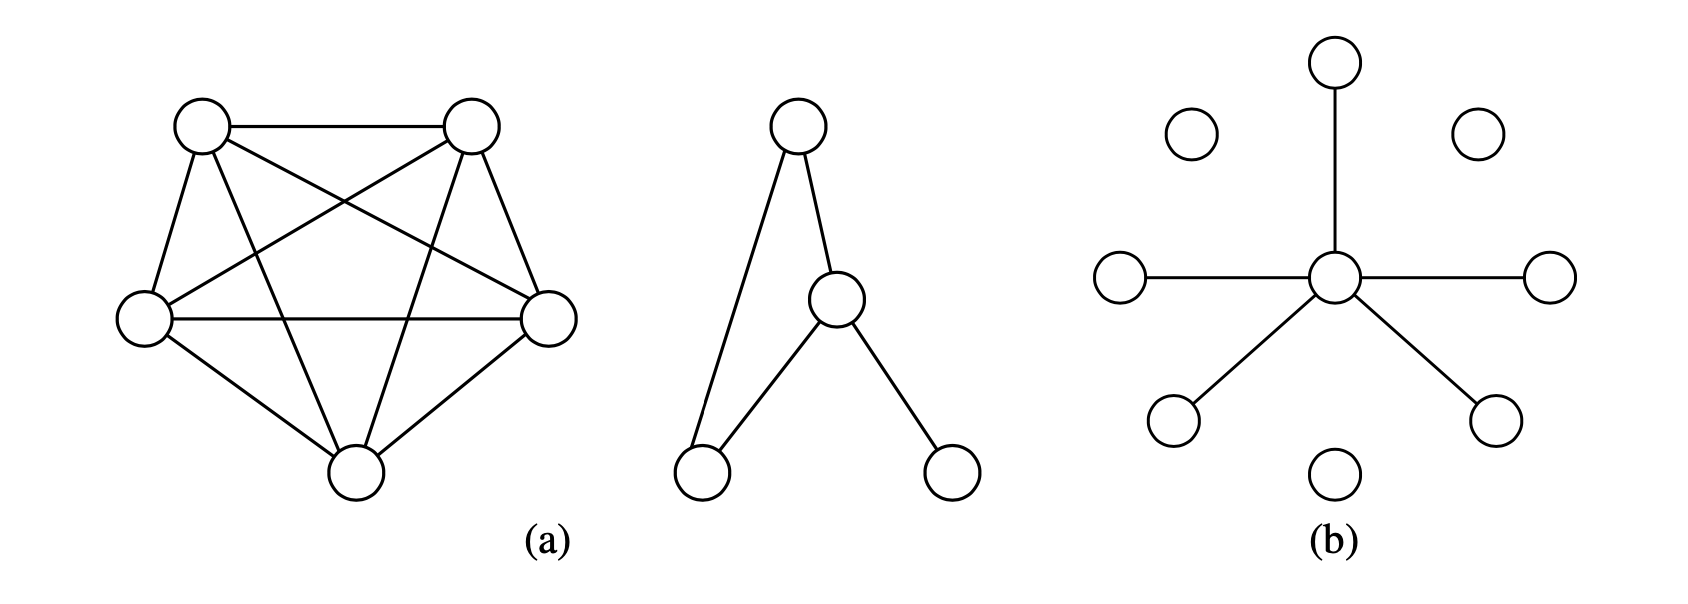
\includegraphics[width=7cm]{figure_6_1.png}
  \end{center}
\end{frame}

\begin{frame}
  \begin{itemize}
    \item Thm6.23の証明のつづき.
    \item (6.54)から, $\widehat{\Delta} := \widehat{\Sigma} - \Sigma$のinfinity normのboundを求めれば良い.
  \end{itemize}
  \begin{block}{Lemma 6.26}
    Thm6.23の条件のもとで, 以下が成り立つ:
    \[
      \bb{P}[\| \widehat{\Delta} \|_{\max} / \sigma^2 \ge t]
      \le 8 e^{-\frac{n}{16}\min\{t, t^2\} + 2 \log d}
      \quad \mathrm{for\ all}\ t > 0.
      \tag{6.56}
    \]
  \end{block}
  \begin{itemize}
    \item (6.56)で $t = \lambda_n / \sigma^2 = 8\sqrt{\frac{\log d}{n}} + \delta$ とすると, $n > \log d$より,
          \[ \bb{P}[\|\widehat{\Delta}\|_{\max} \ge \lambda_n] \le 8e^{-\frac{n}{16}\min\{\delta, \delta^2\}}, \]
          となる.
    \item したがってあとはLemma 6.26を示せばよい.
  \end{itemize}
\end{frame}

\begin{frame}
  \begin{itemize}
    \item $\sigma = 1$として一般性を失わない($x_i/\sigma$はsub-Gaussian w/ at most $1$ なので, あとでrescaleすればよい).
    \item まず対角成分を考えると, Exercise 6.15(a)より定数$c_1, c_2$が存在して
          \[ \bb{P}[|\widehat{\Delta}_{jj}| \ge c_1\delta] \le 2e^{-c_2 n \delta^2} \quad \mathrm{for\ all} \delta \in (0, 1). \tag{6.57}\]
    \item 非対角成分については次が成り立つ:
          \[
            2 \widehat{\Delta}_{j \ell}
            =\frac{2}{n} \sum_{i=1}^{n} x_{i j} x_{i \ell}-2 \Sigma_{j \ell}
            =\frac{1}{n} \sum_{i=1}^{n}\left(x_{i j}+x_{i \ell}\right)^{2}-\left(\Sigma_{j j}+\Sigma_{\ell \ell}+2 \Sigma_{j \ell}\right)-\widehat{\Delta}_{j j}-\widehat{\Delta}_{\ell \ell}.
          \]
    \item 各$x_{ij}$はzero-mean sub-Gaussian with at most parameter $\sigma$なので, $x_{ij}+x_{i\ell}$はzero-mean sub-Gaussian w/ parameter at most $2\sqrt{2}\sigma$ (see Exercise 2.13).
    \item よって, 定数$c_2, c_3$に対して, 任意の$\delta \in (0,1)$について
          \[
            \bb{P}\left[ \left|\frac{1}{n}\sum_{i=1}^n (x_{ij}+x_{i\ell})^2 - (\Sigma_{jj}+\Sigma_{\ell\ell}+2\Sigma_{j\ell})\right| \ge c_3 \delta \right] \le 2 e^{- c_2 n \delta^2}
          \]
          で, (6.57)と合わせると$\bb{P}[|\widehat{\Delta}_{j\ell}| \ge c_1'\delta] \le 6e^{-c_2 n \delta^2}$となる.
    \item (6.57)と合わせて$d^2$-entryについて合わせると, claim (6.56)を得る.
  \end{itemize}
\end{frame}

\subsection{6.5.2 Approximate sparsity}
\begin{frame}{6.5.2 Approximate sparsity}{}
  \begin{itemize}
    \item Thm 6.23は, 厳密に$0$であるentryが少ない場合は使い物にならない.
    \item 厳密に$0$ではなくとも多くのentryが``near zero''であるときを考える.\\
           \\
    \item $\Sigma$は, パラメータ$q\in[0,1]$と半径$R_q$に対して, 以下を満たすとする:
          \[
            \max_{j = 1,\dots, d} \sum_{\ell = 1}^d |\Sigma_{j\ell}|^q \le R_q.
            \tag{6.58}
          \]
          \begin{itemize}
            \item $q = 0$なら, 各行のnon-zero entryが最大$R_q$であることを示す.
            \item $\Sigma$が(6.58)を満たすとき, $\ell_q$-sparsityを満たすという.
          \end{itemize}
  \end{itemize}
\end{frame}

\begin{frame}
  \begin{block}{Theorem 6.27 (Covariance estimation under $\ell_q$-sparsity)}
    Covariance matrix $\Sigma$ は$\ell_q$-sparsity(6.58)を満たすとする.
    このとき任意の$\lambda_n$ s.t. $\|\widehat{\Sigma} - \Sigma\|_{\max} \le \lambda_n/2$に対して以下が成り立つ:
    \[
      |||T_{\lambda_n}(\widehat{\Sigma}) - \Sigma|||_2 \le 4 R_n \lambda_n^{1-q}.
      \tag{6.59a}
    \]
    $\{x_i\}_{i=1}^n$はzero-meanでsub-Gaussian w/ parameter at most $\sigma$からのi.i.d.サンプルなら,
    $\lambda_n/\sigma^2 = 8\sqrt{\frac{\log d}{n}} + \delta$として以下が成り立つ:
    \[
      \mathbb{P}\left[\left\|T_{\lambda_{n}}(\widehat{\Sigma})-\Sigma\right\|_{2} \geq 4 R_{q} \lambda_{n}{ }^{1-q}\right]
      \leq 8 e^{-\frac{n}{16} \min \left\{\delta, \delta^{2}\right\}} \quad \text { for all } \delta>0
      \tag{6.59b}
    \]
  \end{block}
\end{frame}

\begin{frame}{}{}
  {\bf Proof.}
  \begin{itemize}
    \item (6.59a)のdeterministic claimをgivenとすると(6.59b)はsub-exponential変数のtail boundから得られるので, (6.59a)を示す.
    \item Exercise 6.2より, operator normは次のようにboundされる:
          \[
            ||| T_{\lambda_n}(\widehat{\Sigma}) - \Sigma|||_2
            \le \max_{j = 1,\dots,d}\sum_{\ell = 1}^d|T_{\lambda_n}(\widehat{\Sigma}_{j\ell}) - \Sigma_{j\ell}|.
          \]
    \item $j \in\{1,\dots,d\}$を固定し, set $S_j(\lambda_n/2) := \{\ell \in \{1,\dots,d\}\mid |\Sigma_{j\ell} > \lambda_n/2|\}$とする.
    \item 任意の$\ell \in S_j(\lambda_n/2)$について,
          \[
            \left|T_{\lambda_{n}}\left(\widehat{\Sigma}_{j \ell}\right)-\Sigma_{j \ell}\right|
            \leq\left|T_{\lambda_{n}}\left(\widehat{\Sigma}_{j \ell}\right)-\widehat{\Sigma}_{j \ell}\right|+\left|\widehat{\Sigma}_{j \ell}-\Sigma_{j \ell}\right|
            \leq \frac{3}{2} \lambda_{n}.
          \]
    \item 一方 $\ell \notin S_j(\lambda_n/2)$ については, $T_{\lambda_n}(\Sigma_{j\ell}) = 0$なので,
          $
            |T_{\lambda_n}(\widehat{\Sigma}_{j\ell}) - \Sigma_{j\ell}| = |\Sigma_{j\ell}|.
          $
    \item したがって, 
          \[
            \sum_{\ell = 1}^d |T_{\lambda_n}(\widehat{\Sigma}_{j\ell} - \Sigma_{j\ell}|
            \le |S_j(\lambda_n/2)|\frac{3}{2}\lambda_n + \sum_{\ell \notin S_j(\lambda_n/2)}|\Sigma_{j\ell}|.
            \tag{6.60}
          \]
  \end{itemize}
\end{frame}

\begin{frame}{}{}
  \begin{itemize}
    \item ここで次が成り立つ:
          \[
            \sum_{\ell \notin S_{j}\left(\lambda_{n} / 2\right)}\left|\Sigma_{j \ell}\right|
            =\frac{\lambda_{n}}{2} \sum_{\ell \notin S_{j}\left(\lambda_{n} / 2\right)} \frac{\left|\Sigma_{j \ell}\right|}{\lambda_{n} / 2}
            \stackrel{\mathrm{(i)}}{\leq} \frac{\lambda_{n}}{2} \sum_{\ell \notin S_{j}\left(\lambda_{n / 2)}\right.}\left(\frac{\left|\Sigma_{j \ell}\right|}{\lambda_{n} / 2}\right)^{q}
            \stackrel{\mathrm{(ii)}}{\leq} \lambda_{n}^{1-q} R_{q}
          \]
          ただし(i)は$|\Sigma_{j\ell}|\le \lambda_n/2$と$q \in [0,1]$より, (ii)は$\ell_q$-sparsityから.
    \item 一方$S_j(\lambda_n/2)$と$\ell_q$-sparsityから,
          \[
            |S_j(\lambda_n / 2)| \le \left(\frac{\lambda_n}{2}\right)^{-q}R_n.
          \]
    \item よって, (6.60)は
          \[
            \sum_{\ell = 1}^d |T_{\lambda_n}(\widehat{\Sigma}_{j\ell} - \Sigma_{j\ell}|
            \le 2^qR_q\lambda_n^{1-q}\frac{3}{2} + R_q \lambda_n^{1-q}
            \le 4 R_q \lambda_n^{1-q}
          \]
          となる.
    \item これが全ての$j \in \{1,\dots,d\}$に対して成立するので, (6.59a)が示された.\qed
  \end{itemize}
\end{frame}

\end{document}
